%%%%%%%%%%%%%%%%%%%%%%%%%%%%%%%%%%%%%%%%%
% Beamer Presentation
% LaTeX Template
% Version 1.0 (10/11/12)
%
% This template has been downloaded from:
% http://www.LaTeXTemplates.com
%
% License:
% CC BY-NC-SA 3.0 (http://creativecommons.org/licenses/by-nc-sa/3.0/)
%
%%%%%%%%%%%%%%%%%%%%%%%%%%%%%%%%%%%%%%%%%

%----------------------------------------------------------------------------------------
%	PACKAGES AND THEMES
%----------------------------------------------------------------------------------------

\documentclass{beamer}

\mode<presentation> {
	
	% The Beamer class comes with a number of default slide themes
	% which change the colors and layouts of slides. Below this is a list
	% of all the themes, uncomment each in turn to see what they look like.
	
	%\usetheme{default}
	%\usetheme{AnnArbor}
	%\usetheme{Antibes}
	%\usetheme{Bergen}
	%\usetheme{Berkeley}
	%\usetheme{Berlin}
	%\usetheme{Boadilla}
	%\usetheme{CambridgeUS}
	%\usetheme{Copenhagen}
	%\usetheme{Darmstadt}
	%\usetheme{Dresden}
	%\usetheme{Frankfurt}
	%\usetheme{Goettingen}
	%\usetheme{Hannover}
	%\usetheme{Ilmenau}
	%\usetheme{JuanLesPins}
	%\usetheme{Luebeck}
	\usetheme{Madrid}
	%\usetheme{Malmoe}
	%\usetheme{Marburg}
	%\usetheme{Montpellier}
	%\usetheme{PaloAlto}
	%\usetheme{Pittsburgh}
	%\usetheme{Rochester}
	%\usetheme{Singapore}
	%\usetheme{Szeged}
	%\usetheme{Warsaw}
	
	% As well as themes, the Beamer class has a number of color themes
	% for any slide theme. Uncomment each of these in turn to see how it
	% changes the colors of your current slide theme.
	
	%\usecolortheme{albatross}
	%\usecolortheme{beaver}
	%\usecolortheme{beetle}
	%\usecolortheme{crane}
	%\usecolortheme{dolphin}
	%\usecolortheme{dove}
	%\usecolortheme{fly}
	%\usecolortheme{lily}
	%\usecolortheme{orchid}
	%\usecolortheme{rose}
	%\usecolortheme{seagull}
	%\usecolortheme{seahorse}
	%\usecolortheme{whale}
	%\usecolortheme{wolverine}
	
	\setbeamertemplate{footline} % To remove the footer line in all slides uncomment this line
	%\setbeamertemplate{footline}[page number] % To replace the footer line in all slides with a simple slide count uncomment this line
	
	\setbeamertemplate{navigation symbols}{} % To remove the navigation symbols from the bottom of all slides uncomment this line
}

\usepackage{graphicx} % Allows including images
\usepackage{booktabs} % Allows the use of \toprule, \midrule and \bottomrule in tables

\usepackage{color}
\definecolor{red}{rgb}{1.0,0.,0.}
\newcommand{\todo}[1]{\textcolor{red}{[[#1]]}}
\usepackage{subfigure}
\usepackage{multicol}


%----------------------------------------------------------------------------------------
%	TITLE PAGE
%----------------------------------------------------------------------------------------

\title[GPU polynomial computation]{Polynomial Computation on GPU} % The short title appears at the bottom of every slide, the full title is only on the title page

\author{Kevin Mueller} % Your name
\institute[UW] % Your institution as it will appear on the bottom of every slide, may be shorthand to save space
{
	\\ % Your institution for the title page
	\medskip
}
\date{\today} % Date, can be changed to a custom date

\begin{document}
	
	\begin{frame}
		\maketitle
	
		
	\end{frame}
	
	\section{Test section one}
	\begin{frame}{Outline}
	
		\vspace{0.2in}
		\begin{itemize}
			\item Overview of Process
			\item Setup
			\item Homomorphisms (Mod Reduction)
			\item Interpolation 
			\item Evaluation (Kernel)
			\item Problems encountered
			\item Extensions (Multivariate)
			\item Demo
		\end{itemize}
		
	\end{frame}
	
	
	\begin{frame}{	Overview of Process}

	
	
		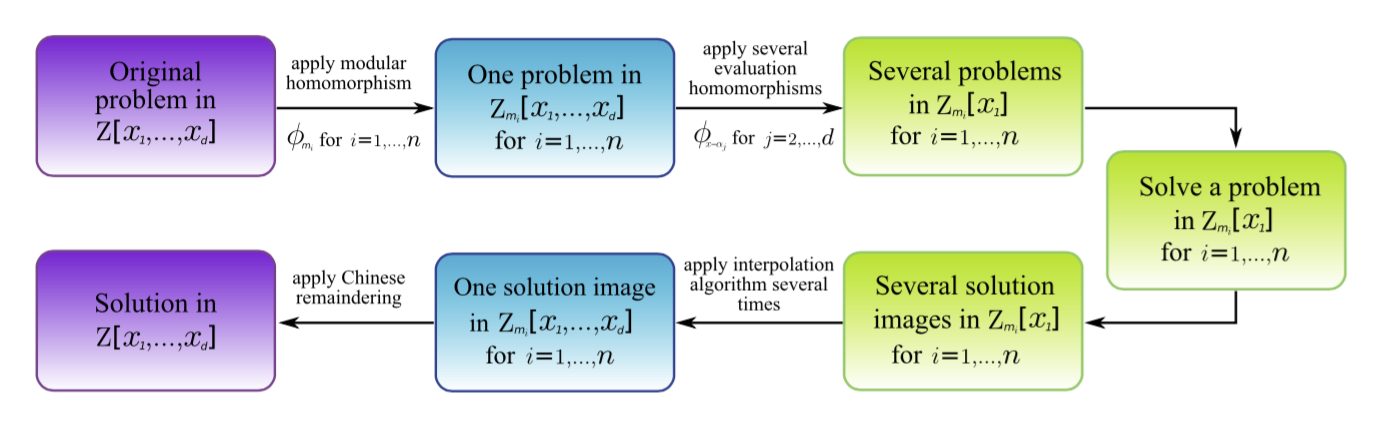
\includegraphics[width=0.995\textwidth]{../Code/Images/diagram_homomorphisms.png}
	
	\end{frame}
	

	
	\begin{frame}{Initial problem Setup}
		
		Suppose we have two polynomials $a(x) = 7x+5,b(x)=2x-3$ and we wish to multiply them  such that
		$$ c(x) = a(x)b(x)$$
		
		We first need to compute bounds for our modular design
		
		\begin{itemize}
			\item Compute upper bound M such that our set of moduli $\prod{m_i} \geq 2M$\\
			\item For multiplication of two polynomials this is M = $2||a||_\infty ||b||_\infty$\\
				$$(7)(3)(2)(2) = 84$$
			Therefore we can take $m = 3,5,7$. However for this problem we will use $m=5,7$ for simplicity.
			\item Compute maximum degree for result polynomial $$\deg (c) = \deg (a) + \deg (b)$$
		\end{itemize}
	\end{frame}
	
	\begin{frame}{Homomorphisms}
		
		
		
		There are two types of homomorphisms we will be dealing with:
		
		\begin{itemize}
			\item Moduluar: $\Phi_m : \mathbf{Z}[x_1,\dots,x_v] \rightarrow \mathbf{Z}_m[x_1,\dots,x_v ]$ \\
			\item In practice this simply means to take the mod on all the coefficients in the polynomial for some prime $m_i$. Such as
			$$a_5(x) = 2x+0 \quad b_5(x)  = 2x + 2$$
			\item Evaluation: $\Phi_{x_i-\alpha} : \mathbf{D}[x_1,\dots,x_v] \rightarrow \mathbf{D}[x_1,\dots,x_{i-1},x_{i+1},\dots,x_v]$
			\item This implies to evaluate each modular polynomial at each evaluation point. For a few examples:
			$$a_5(0) = 0 \quad b_5(0) = 2$$		
			
		
		\end{itemize}
					
	\end{frame}
	

	
	\begin{frame}{Interpolation}
	

		We can solve the interpolation problem with the vandermonde matrix $ \mathbf{V} $ as
		
		$$\mathbf{V} \mathbf{a} = \mathbf{b}  $$
		
		where $n$ is the number of evaluation points, $\mathbf{V}$ is the Vandermonde matrix with $(i,j)$-th entry $\alpha_i^j(i,j=0,1,\dots,n)$, $\mathbf{b}$ is the vector with the $i$-th entry $b_i(i=0,1,\dots,n)$, and $\mathbf{a}$ is the vector of unknown coefficients $a_i(i=0,1,\dots,n)$.
		
		\[\left( \begin{array}{l}
		{c_5}(0) = 0\bmod 5\\
		{c_5}(1) = 3\bmod 5\\
		{c_5}(2) = 4\bmod 5
		\end{array} \right) \to {c_5}(x) = 4{x^2} + 4x\]
				
		\[\left( \begin{array}{l}
		{c_7}(0) = 6\bmod 7\\
		{c_7}(1) = 2\bmod 7\\
		{c_7}(2) = 5\bmod 7
		\end{array} \right) \to {c_7}(x) = 3x + 6\]
		
		
		
	\end{frame}
	
	\begin{frame}{Chinese Remaindering}
		
		For a set of residues $r_i \in \mathbb{Z}(1\leq i \leq k)$ and a set of positive prime moduli $m_i \in \mathbb{Z}_{m_i}(1 \leq i \leq k)$, we can compute a unique $u \in \mathbb{Z}_m$ in the mixed radix form  as
		
		$$u = v_1 + v_2(m_1) + v(m_0m_1) + \dots + v_n\left( \prod_{i=0}^{k-1}m_i \right)  $$
		
		Which we can rewrite the 2nd coefficient as $M_1 = 1, M_i = m_1m_2\dots m_{i-1}(i=2,\dots,k)$. Satisfying the system of congruences gives us
		
		\begin{align*}
		v_1 &= r_1 \\
		v_2 &= (r2-v_1)\gamma_2 \mod m_2\\
		v_i &= ((r_i-v_1)\gamma_i - (\gamma_2M_2c_i \mod m_i) - \dots -(v_{i-1}M_{i-1}\gamma_i \mod{m_i}))
		\end{align*}
		
	
		\end{frame}
		
		\begin{frame}{Chinese Remaindering continued}
			
			In practice we will precompute the coefficients as $$\gamma_i = (m_1m_2\dots m_{i-1})^{-1} \mod{m_i}$$.
			
			Finally we can recover the full integer $r$ using the recursion
			$$ r = \gamma_1 + m_1(\gamma_2 + m_2(\gamma_3 + m_3(\dots)))$$.
		\end{frame}	
		\begin{frame}
			\vspace{0.0in}
			\begin{figure}
				\centering
				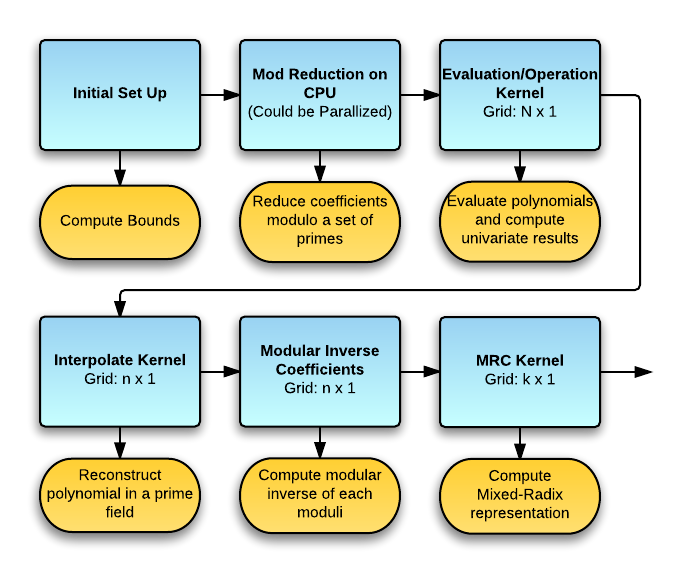
\includegraphics[scale=0.40]{../Code/Images/FlowCUDAPoly3.png}
				\caption{k: Number of Moduli, n: Number of Evaluation Points}	
			\end{figure}
		\end{frame}	
		
		
	\begin{frame}{Evaluation Kernel Implementation}
		After performing all the modular homomorphisms necessary we want to maximize threads used to evaluate the polynomials in field $\mathbf{Z}_{m_i}$. In order to accomplish this we will need to vectorize all the coefficients and perform detailed bookkeeping to correctly index this coefficient vector $X$. We can then find the resulting vector $Y \in \mathbb{Z}^N$ as
		
		$$Y_i = a_{j}\alpha^\theta$$,
		
		Where $\theta = \left(i \mod d\right)$, $j = \theta  + d \cdot \text{quo}(i,n /cdot d)$ and 
		$\alpha = \text{quo}\left(\left(i\mod nd\right),d\right)$ when
		
		%and $l$ is the number of polynomials, $k = \text{len}(m)$ is the number of moduli, $n = \deg c+ 1$ is the number of evaluation points and $d= \max\left\{\deg( a(x)),\deg(b(x))\right\}$.
		
		\begin{itemize}
		\item $l$ is the number of polynomials (i.e 2) \\
		\item $k = \text{len}(m)$  \\
		\item $n = \deg(c)+ 1$ \\
		\item $d= \max\left\{\deg( a(x)),\deg(b(x))\right\}$\\
		\item $N = l \cdot k \cdot n\cdot d$
		\end{itemize}
		
		
		
	\end{frame}
		
			 

	\begin{frame}{Problems Encountered}
		\begin{itemize}
			\item Filling in zeros for coefficients with missing terms and handling string representations. Python libraries had poor support for this
			\item Python CUDA wrapper/compiler lacks some low level functionality.
			\item Coefficient swell in newton interpolation.  \\
			\item Ill-conditioned Vandermonde matrix.
			\item Potential trade off between different polynomial representations.
			\item Sparsity required for operations in polynomial domain.
			\item Operation kernels for more complicated operations (division,GCD,resultant,etc).
		\end{itemize}
	\end{frame}
	
	\begin{frame}{Extensions}
		There is a natural tendency to want to extend the above schemes into the multivariate domain. This seems somewhat straightforward since,
		
		$$ \mathbf{D}[x_3] \xrightarrow{\Phi_{x_2-\alpha}} \mathbf{D}[x_2,x_3] \xrightarrow{\Phi_{x_1-\alpha}} \mathbf{D}[x_1,x_2,x_3] $$
					
		%
		That is, each multivariate problem can be decomposed into a set of univariate interpolation problems where one evaluation homomorphism $\Phi_{x_i-\alpha}$ is inverted at a time. However the interpolation becomes slightly less straight forward and sparsity becomes an even bigger issue.
		
		A few other possible extensions could be:
		\begin{itemize}
		\item Perform the mod reductions on GPU \\
		\item Implement a parallel newton interpolation kernel
		\item Better support for mathematica
		\end{itemize}		
		
				
		
	\end{frame}
	
	

	
	
	
	
	
	%------------------------------------------------
	
	\begin{frame}
		\frametitle{References}
		\footnotesize{
			\begin{thebibliography}{99} % Beamer does not support BibTeX so references must be inserted manually as below
				\bibitem[FF]{p1} Keith Geddes
				\newblock Algorithms For Computer Algebra
				
				\bibitem[GW]{p1} Pavel Emeliyanenko
				\newblock Harnessing the Power of GPUs for Problems in Real Algebraic Geometry.
				\newblock \emph{PhD thesis, Universität des Saarlandes, 2012} 
			\end{thebibliography}
		}
	\end{frame}
	
\end{document} 